\documentclass[german,12pt,a4paper]{article}
\usepackage{fullpage}
\usepackage[ngerman]{babel}
\usepackage[utf8]{inputenc}
\usepackage{listings}
\usepackage{verbatim}
\usepackage{enumerate}
\usepackage{graphicx}
\usepackage{float}
\usepackage{wrapfig}
\usepackage{color}
\usepackage[usenames,dvipsnames]{xcolor}
\usepackage[font=small,format=plain,labelfont=bf,up,textfont=it,up]{caption}
\usepackage{subfig}
\usepackage[colorlinks=false,pdfborder={0 0 0}]{hyperref}
\usepackage{eurosym}

\bibliographystyle{plain}
\pagestyle{plain}
\pagenumbering{arabic}
\frenchspacing

\newcommand{\comments}[1]{}
\renewcommand{\baselinestretch}{1.6}

%Redefine the first level
\renewcommand{\theenumi}{\textbf{\alph{enumi})}}
\renewcommand{\labelenumi}{\theenumi}

\begin{document}

\title{\textbf{SMS in Datennetzen}}
\author{Sebastian Menski (734272), Martin Ohmann (734801) \\ \texttt{\{menski,ohmann\}@uni-potsdam.de}}
\date{\today}

\maketitle

\begin{abstract}
In dieser Arbeit geht es um die Gegenüberstellung des Short Message Service 
GSM-Standards mit SMS-Alternativen, welche mobile Datennetze als Übertragungskanal 
nutzen. Dazu wird die Funktionsweise von SMS über GSM und der Rich Communication Suite enhanced 
-- einer SMS-Realisierung über Datennetze -- verglichen und ein Überblick über die Nachteile 
von SMS über GSM gegeben. Zusätzlich werden weitere SMS-Alternativen aufgezeigt und gegenübergestellt.
\end{abstract}

\section{Einleitung}
Einleitung

\section{Geschichte}
Erste Überlegungen zu einem Textnachrichtendienst gab es bereits 1984 bei den 
europäischen Telekommunikationsgesellschaften. Damals wurde der ursprüngliche 
Konzeptvorschlag für den Short Message Service von Friedhelm Hillebrand von der 
damaligen Deutschen Bundespost mit Beiträgen von Bernard Ghillebaert von der PTT 
(Vorgänger der france Télécom) erarbeitet und schließlich 1985 in die 
GSM-Standarisierung eingebracht. Die erste Version des endgültigen Standards 
wurde 1989 verabschiedet. Finn Trosby von der norwegischen Telenor war es, der 
1987 bis 1990 als Leiter der Standardisierungsgruppe GSM4 DGMH (Drafting Group 
Message Handling) mit dieser das erste technische Design erarbeitete und 
standardisierte.
Vorn 1990 bis 2009 wurde der SMS-Standard in dieser Gruppe unter Leitung von 
Kevin Holly von Cellnet und Ian Harris von Vodafone weiterentwickelt\cite{wikipedia:sms}.

Die erste Kurzmitteilung des Short Message Service wurde am 3. Dezember 1992 
von einem PC an ein Mobiltelefon im britischen Vodafone-Netz gesendet. Dies 
war etwa ein Jahr nach der Einführung des GSM-Standards für Mobiltelefone in 
Europa.

\section{SMS über GSM} % {{{
\subsection{Spezifikation}
SMS-Nachrichten werden durch das \textit{Short Message Service Center} (SMSC) des 
Providers verwaltet. Nachrichten werden vom Endgerät über Funk via dem 
Funkturm der Mobilfunkzelle an das SMSC gesendet und umgekehrt. Die 
Zugriffsprotokolle des SMSCs erlauben Interaktionen zwischen zwei SMSCs oder 
zwischen externen \textit{Short Message Entities} (SMEs) und einem SMSC. SMEs sind 
Software-Anwendungen auf Netzwerkkomponenten oder Hardware-Geräte, welche SMS
senden und empfangen können. Das \textit{Short Message Peer-to-Peer Protocol} (SMPP) 
wird hierbei für die Interaktion zwischen SMEs und SMSCs verschiedener 
Hersteller genutzt\cite{thesms}.

\begin{figure}[htm]
    \centering
	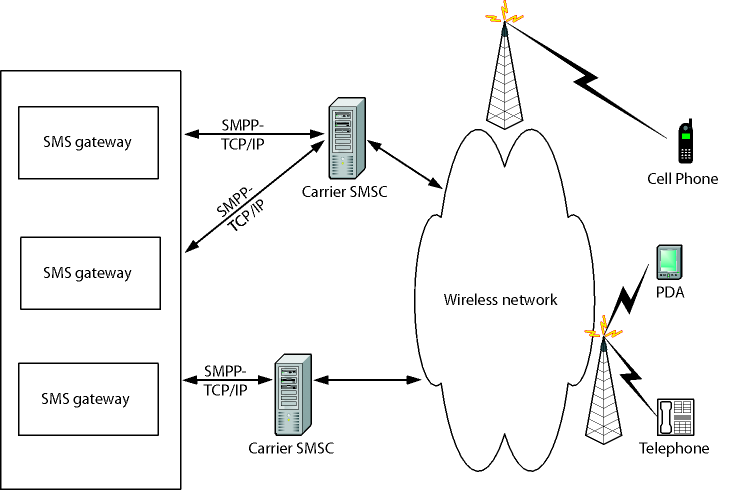
\includegraphics[width=0.9\textwidth]{img/smspp.png}
    \label{fig:smspp}
    \caption{Interaktionen zwischen SMSCs und SMEs}
\end{figure}	

Das SMSC arbeitet dabei entweder nach dem \textit{Store-and-Forward} oder 
\textit{Forward-and-Forget}-Prinzip. Beim \textit{Store-and-Forward}-Prinzip versucht das System 
die Nachricht regelmäßig für eine festgelegte Vorhaltezeit an den Empfänger 
zu übermitteln, bis diese erfolgreich bei ihm eingetroffen ist\cite{held:down}. Nachrichten, die innnerhalb 
der Vorhaltezeit nicht zugestellt werden konnten, werden von SMSC gelöscht. 
Ist die Empfängernummer dem SMSC unbekannt, lehnt es diese sofort an.
Arbeitet das SMSC nach dem \textit{Forward-and-Forget}-Prinzip, dann werden Nachrichten ohne 
Zwischenspeicherung an den Empfänger weitergeleitet. Es erfolgt hierbei keine Prüfung, 
ob die Nachricht auch tatsächlich angekommen ist. In der Regel wird von SMSCs überwiegend 
das \textit{Store-and-Forward}-Prinzip benutzt.

Eine SMS-Nachricht kann gewöhnlich bis zu 160 7-Bit-kodierte Zeichen beinhalten. 
Es sind jedoch auch 8-Bit- und 16-Bit-Kodierungen möglich. Hierbei beträgt die 
maximale Nachrichtenlänge 140 bzw. 70 Zeichen\cite{thesms}. 

SMS können auch dazu benutzt werden Binärdaten zu senden, wie zum Beispiel 
Klingeltöne oder Bildnachrichten. Spezielle Anwendungen auf 
dem Telefon übernehmen die Verarbeitung Dieser.


% \begin{figure}[h!]
%     \centering
%     \begin{tabular}{ p{4cm} | p{10cm} }
%         \textbf{Oktett(s)} & \textbf{Beschreibung} \\
%         \hline \hline
%          \texttt{07} & Länge der SMSC-Informationen (hier 7 Oktetts) \\ 
%          \hline
%          \texttt{91} & Typ der SMSC-Adresse (91 bedeutet internationales Telefonnummernformat) \\ 
%          \hline
%          \texttt{72 83 01 00 10 F5} & SMSC-Nummer (hier +27381000015) \\ 
%          \hline
%          \texttt{04} & Erstes Oktett dieser SMS-DELIVER message \\ 
%          \hline
%          \texttt{0B} & Länge der Adresse/Nummer des Senders (0B$_{16}$ = 11$_{10}$) \\ 
%          \hline
%          \texttt{C8} & Typ der Sender-Adresse \\ 
%          \hline
%          \texttt{72 38 88 09 00 F1} & Sender-Nummer (hier +27838890001) \\ 
%          \hline
%          \texttt{00} & Protocol identifier (00 = SME-to-SME Protokoll -- implizit) \\ 
%          \hline
%          \texttt{00} & Datenkodierung (00 = 7 bit, 01 = 8 bit, 10 = 16 bit, 11 = reserviert) \\ 
%          \hline
%          \texttt{99 30 92 51 61 95 80} & Zeitstempel \\ 
%          \hline
%          \texttt{0A} & Nutzdatenlänge/Länge der Nachricht \\ 
%          \hline
%          \texttt{E8 32 9B FD 46 97 D9 EC 37} & Nachricht "hellohello", 8-bit Oktetts representiert als 7-bit Daten
%     \end{tabular}
%     \label{tbl:sms-struct}
%     \centering
%     \caption{Beispiel der Transfer Protocol Data Unit: 
%         \texttt{07 91 72 83 01 00 10 F5 04 0B C8 72 38 88 09 00 F1 00 00 99 30 92 51 61 95 80 0A E8 32 9B FD 46 97 D9 EC 37}
%     }
% \end{figure}

\subsection{Nachrichtentypen}
Neben den normalen Kurznachrichten bietet der SMS-Standard noch drei weitere Textnachrichtentypen:
\begin{itemize}
	\item \textbf{Flash Message:} erscheint direkt auf Display des Empfängers. Die meisten Mobiltelefone 
        können solche Nachrichten nicht speichern. Ein Anwendungsbeispiel für solche Flash Messages ist die 
        Anzeige des Restguthabens direkt nach einem Gespräch.
	\item \textbf{Silent Message:} erscheinen weder auf dem Display noch durch akkustisches Signal. 
		Silent Messages werden z.B. von Polizei und Geheimdiensten zur Personenortung genutzt.
	\item \textbf{Concatenated Message:} Das System ist in der Lage überlange 
Nachrichten zu segmentieren. So werden bei Nachrichten, die länger als 160 Zeichen 
sind, mehrere SMS gesendet und später beim Empfänger wieder zusammengesetzt.
\end{itemize}

\subsection{Übertragung}
Zur Übertragung nutzt der Short Message Service nutzt einen Signalisierungskanel des GSM-Standards wie etwa SDCCH 
(\textit{Stand-alone Dedicated Control Channel}) oder FACCH (\textit{Fast Associated Control Channel}). 
Diese Kanäle werden auch genutzt, um Gespräche aufzubauen und zu halten.

Kurzmitteilungen können parallel zu Telefongesprächen empfangen/gesendet werden. Teil der Bandbreite des 
Verkehrsdatenkanals wird hier temporär zum Signailiserungskanal (SACCH) umkonfiguriert\cite{wikipedia:sms}.


\subsection{Technische Realisierung über GSM}
Der Short Message Service wird durch den \textit{Mobile Application Part} (MAP) des SS\#7 Protokolls (\textit{Signaling 
System No. 7}) realisiert\cite{3gpp:map}. Die Elemente des Short Message Protokolls werden als Felder innerhalb von 
MAP-Nachrichten durch das Netzwerk transportiert. Bei der Übertragung von Kurznachrichten vom Empfänger zum
Service Center wird die Prozedur \textit{Mobile Originated (MO) Short Message Service Transfer} genutzt,
für die Übertragung vom Service Center zum Empfänger die Prozedur \textit{Mobile Terminated (MT) Short
Message Service Transfer}. Zum Abhandeln von Fehlern und Verwalten von Warteschlangen stehen zudem die 
Prozeduren \textit{Short Message Alert} und \textit{Short Message Waiting Data Set} 
zur Verfügung\cite{3gpp:map}. Die Funktionsweise dieser Prozeduren wird im folgenden genauer beschrieben.


\subsubsection{Mobile Originated Short Message Service Transfer}
Immer wenn ein Nutzer eine SMS versendet, wird diese zum nächsten VMSC/SGSN (\textit{Mobile Switching 
Center/GPRS Core Network}) gesendet. Neben der Textnachricht werden Zieladresse und die Adresse des 
SMSCs übermittelt. 

Die Adresse des SMSCs ist hierbei in der Telefonkonfiguration der SIM-Karte definiert\cite{3gpp:smpp}. Das VMSC/SGSN 
ruft das MAP service package \textit{MAP\_MO\_FORWARD\_SHORT\_\-MESSAGE} auf um die Nachricht an das spezifizierte 
\textit{Interworking MSC} des Service Centers zu senden. Der Service sendet die \textit{mo-ForwardSM} MAP-Operation --
eingebettet in den \textit{Transaction Capabilities Application Part (TCAP)} -- an das SMSC, welches in der 
Nachricht angegeben wurde. Der Transport erfolgt hierbei über das \textit{Core Network} mittels des \textit{Signaling 
Connection Control Parts} (SCCP)\cite{3gpp:smpp}.

\begin{figure}[htm]
    \centering
	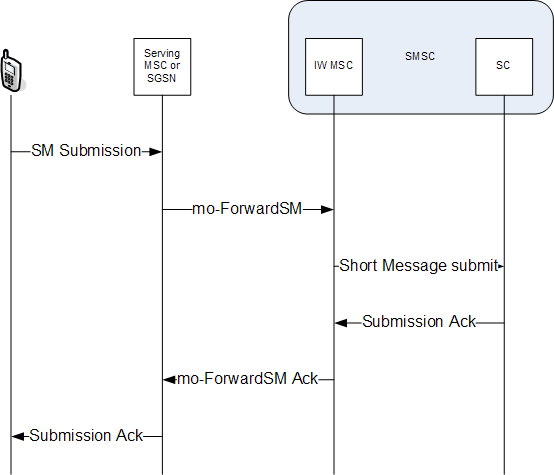
\includegraphics[width=0.9\textwidth]{img/mo-forward-sm.png}
    \label{fig:mo-forward-sm}
    \caption{Transport einer Kurznachricht vom Sender zum Service Center}
\end{figure}	

Nach Erhalt der \textit{mo-ForwardSM} MAP-Nachricht gibt das \textit{Interworking MSC} des SMSC die SMS-PP \textit{Application 
Protocol Data Unit} (APDU) (beinhaltet den Nachrichtentext) an das zuständige Service Center des SMSC 
weiter\cite{3gpp:techrel}. Hier wird sie gespeichert und anschließend versucht an die Zieladresse auszuliefern. Das 
Service Center liefert als Submission Status eine Erfolgs- oder Fehlermeldung zurück.

Nach Erhalt des Submission Status vom Service Center sendet das \textit{Interworking MSC} eine Benachrichtigung
zurück an das VMSC/SGSN des Senders. Von dort aus wird die Benachrichtigung über Funk an den Sender
ausgeliefert.


\subsubsection{Mobile Terminated Short Message Service Transfer}
Wenn das SMSC feststellt, dass es eine SMS ausliefern soll, dann sendet es die SMS-PP APDU der Nachricht 
an die \textit{Gateway MSC} (GMSC) Komponente des SMSC\cite{3gpp:techrel}. Das GMSC muss nach dem Empfangen der Nachricht die Position
des Empfängers herausfinden (in diesem Zusammenahng ist der Begriff \textit{Gateway MSC} ein \textit{Mobile Switching Center}, das Routing 
Informationen aus dem \textit{Home Location Register} (HLR) bezieht). Dies geschieht, indem das GMSC das MAP-Servicepaket 
\textit{MAP\_SEND\_ROUTING\_INFO\_FOR\_SM} aufruft, welches eine \textit{sendRoutingInfoForSM} (SRI-for-SM) 
MAP-Nachricht an das HLR der Zielnummer sendet, um die aktuelle Position des Empfängers anzufragen.
Die SRI-for-SM-Nachricht kann entweder an ein HLR im gleichen Netzwerk, oder aber über eine Verbindung zu
einem HLR in einem fremden PLMN (\textit{Public Land Mobile Network}) gesendet werden, je nachdem zu welchem 
Netzwerk der Empfänger gehört.

Das HLR führt eine Datenbanksuche durch und sendet die Daten zur aktuellen Position des Empfängers an das 
GMSC des SMSCs zurück. Diese Positionsdaten können entweder die Adresse des \textit{Mobile Switching Centers} sein, über welches der 
Empfänger gerade erreichbar ist, die SGSN Adresse, oder beides. Das HLR kann ebenfalls eine Fehlermeldung 
zurücksenden, fall der Empfänger nicht für Kurznachrichten geeignet ist.

Sobald das GMSC die Routing Informationen erhalten hat, versucht es die Nachricht an den Empfänger zu 
übermitteln. Diese geschieht die das Aufrufen des \textit{MAP\_MT\_\-FORWARD\_SHORT\_MESSAGE} Services, welcher eine
\textit{mt-ForwardSM} MAP-Nachricht an die vom HLR bereitgestellte Adresse sendet. Dabei ist es egal, ob es sich 
hierbei um ein MSC oder SGSN handelt.

Das VMSC fragt die benötigten Informationen zum Ausliefern der Nachricht beim \textit{Visitor Location Register}
(VLR) durch eine \textit{Send\_Infor\_for\_MS\_SMS} Nachricht ab. Das VLR sucht daraufhin nach dem Empfänger und
liefert die \textit{Mobile Subscriber ISDN Number} (MSISDN) des Empfängers an das VMSC zurück. Im Fehlerfall wird 
eine Benachrichtigung an das VMSC gesendet, die Auslieferung des SMS abgebrochen, und der gescheiterte 
Zustellversuch beim SMSC gemeldet. Em Erfolgsfall sendet das VMSC eine Erfolgsnachricht an das SMSC.

Die GMSC Komponente des SMSC reicht das Ergebnis des Zustellversuchs an das Service Center weiter. Im
Erfolgsfall wird die Nachricht aus der \textit{Store and Forward Engine} (SFE) entfernt und -- falls angefordert --
ein Zustellreport an den Sender geschickt\cite{3gpp:techrel}. Bei einem gescheiterten Zustellversuch versucht das SMSC
periodisch die Nachricht für eine bestimmte Vorhaltezeit zuzstellen. Das SMSC registiert sich eventuell 
beim HLR, um über eine erneute Verfügbarkeit des Empfängers benachrichtigt zu werden.

\begin{figure}[htm]
    \centering
	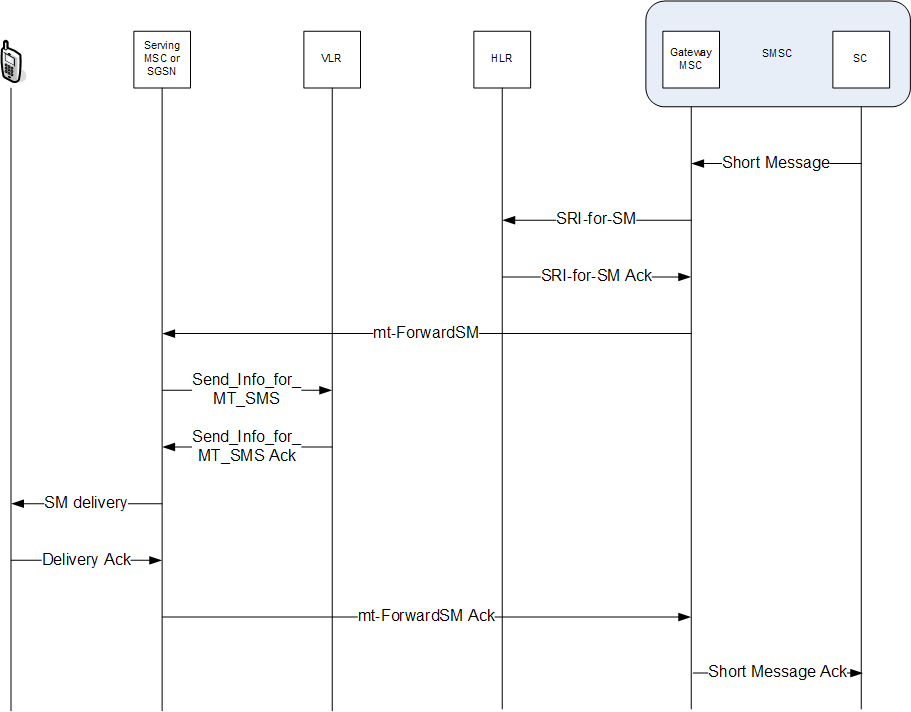
\includegraphics[width=0.9\textwidth]{img/mt-forward-sm.png}
    \label{fig:mt-forward-sm}
    \caption{Transport einer Kurznachricht vom Service Center zum Empfänger}
\end{figure}	

\subsubsection{Gescheiterte Zustellung und Warteschlange}
Falls das SMSC/SGSN einen Fehler bei der Auslieferung anzeigt, dann sendet das SMSC mit Hilfe der 
MAP-Prozedur \textit{MAP\_REPORT\_SM\_DELIVERY\_STATUS} eine Nachricht an das HLR, welche den Grund des Fehlers
angeibt und zusätzlich eine Anfrage zur automatischen Benachrichtigung des SMSC durch das HLR über die 
Zieladresse stellt.

Das HLR setzt ein Flag für den Zielaccount, welches angibt, dass dieser momentan für die Übermittlung von 
Kurznachrichten nicht verfügbar ist und speichert die Adresse des SMSCs in der \textit{Message Waiting Data} (MWD) 
Liste des Ziels. Gültige Flags sind hierbei: \textit{Mobile Not Reachable} (MNRF), \textit{Memory Capacity Exceeded} (MCEF) und
\textit{Mobile Not Reachable for GPRS} (MNRG). Ab diesem Zeitpunkt antwortet das HLR auf SRI-for-SM-Anfragen mit 
einem Fehler und fügt die Adressen der anfragenden SMSC automatisch der MWD-Liste des Ziel hinzu. Sollte 
eine SRI-for-SM-Anfrage ein gesetztes Priority Flag haben, dann antwortet das HLR mit der VLR-Adresse, 
falls diese verfügbar ist.

Das HR kann auf verschiedenen Wegen über die erneute Verfügbarkeit für Kurznachrichten eines Teilnehmers 
informiert werden:
\begin{itemize}
    \item Der Teilnehmer wurde vom Netzwerk getrennt. Eine Neuverbindung löst ein Location Update beim 
    HLR aus.
    \item Der Teilnehmer befand sich in einem ``Funkloch'', wurde jedoch nicht komplett vom Netzwerk
    getrennt. Beim erneuten Eintritt in einen abgedeckten Netzbereich antwortet es auf Page Requests
    des VLRs. Das VLR sendet daraufhin eine Ready-for-SM Nachricht and das HLR.
    \item Wenn der Telefonspeicher voll war und der Teilnehmer daraufhin einige Nachrichten löscht, so
    wird eine Ready-for-SM-Nachricht vom VMSC/VLR an das HLR gesendet.
\end{itemize}

Sobald das HLR über die erneute Verfügbarkeit des Teilnehmers informiert wurde, sendet es eine AlertSC 
MAP message an jedes in der MWD Liste des Teilnehmers registierte SMSC, wodurch der SMS-Zustellprozess
erneut gestartet wird\cite{3gpp:map}.

% \subsection{Message aggregators}
% \begin{itemize}
% 	\item Provider kommunizieren in der Regel nicht direkt mit SMSCs, sondern nutzen einen SMS Broker (oder message aggregator)
% 	\item Ein Aggregator ist eine Wirtschaftseinheit, welcher Verträge mit Netzwerk-Providern aushandelt und als Mittelsmann
% 		Zugang zu Mobilfunknetzen zur Nachrichtenübertragung für Dritte ohne direkte Beziehung zum Mobilfunknetzwerk gewährt. 
% 	\item Der Aggregator nutzt SMPP um Verbindungen mit Provider-Mobilfunknetzwerken aufrechtzuerhalten.
% 	\item Aggregatoren bieten Zugriff auf ihre Server typischerweise über SMPP oder kundenspezifische APIs an.
% 	\item \textit{Grafik SMSC, SMPP, SMS Broker anführen \\(Computer-SMS\_pdf.pdf, Figure 1)}
% \end{itemize}


\subsection{Nachteile von SMS über GSM}
Mit der voranschreitenden Entwicklung der mobilen Datennetze und Endgeräte ist die klassische SMS über GSM  in vielen Belangen
nicht mehr zeitgemäß und bietet eine ganze Reihe an Nachteilen:
\begin{itemize}
	\item \textbf{Multi-Device:} Der SMS Service ist an eine einzige Mobilfunknummer gebunden, was in der heutigen Zeit -- 
		wo Laptops, Tablets, Smartphones und PCs benutzt werden -- einen großen Nachteil gegenüber SMS Alternativen 
		bildet, welche die Möglichkeit bieten, einen Account auf mehreren Geräten gleichzeitig nutzen zu können.
	\item \textbf{Kosten:} SMS sind teuer. Ein Rechenbeispiel: Geht man von 16 Cents/SMS aus, dann entspricht das bei einer Länge von 
        140 Bytes pro Nachricht Kosten in Höhe von 0.11 Cents pro Byte. Bei einer Datenflat für \EUR{30} pro 2GB entspricht das 
        0.000003 Cents pro Byte. Die Kosten einer Datenflat sind also für den Nutzer wesentlich attraktiver als die Kosten für 
        herkömmliche SMS-Nachrichten.
	\item \textbf{Real-Time:} Es gibt keine Garantie für die Zustellzeit. Die Zustellung kann manchmal viel Zeit in Anspruch nehmen. 
		Desweiteren gibt es kein ``is typing'' Feature, welches aus vielen anderen Messengern bekannt ist. Apple iMessage z.B. bietet 
		dieses Feature und kommt zudem mit geringeren Zustellzeiten aus.
	\item \textbf{Gruppen:} Nachrichten an eine Gruppe von Personen sind in SMS nicht möglich. Es ist zwar möglich, eine Nachricht 
        an mehrere Personen gleichzeitig zu senden, jedoch sind diese voneinander unabhängig. Die Empfänger können nicht sehen, 
        an welche Personen die Nachricht ebenfalls gesendet wurde und haben somit keine Möglichkeit der Gruppe als Ganzes zu antworten.
	\item \textbf{Rich Text:} Die Limitation auf 160 7-Bit Zeichen lässt keine besonderen Formatierungen oder Schriftarten zu. 
        Das Einbetten von Grafiken, Emoticons und anderen Multimediainhalten ist nicht möglich. Enhanced Messaging Service Nachrichten 
        füllen diese Lücke.
	\item \textbf{Übertragungskanal:} Zur Übertragung wird der Signalisierungskanal des GSM-Standards verwendet. Ursprünglich waren 
        SMS-Nachrichten dazu gedacht, Mitteilungen über Netzstörungen oder ähnliche Informationen an den Nutzer zu senden. Dementsprechend 
        wurde der Übertragungskanal für das heutige Aufkommen an SMS-Nachrichten nicht ausgelegt.
\end{itemize}

In den letzten Jahren haben sich viele SMS-Alternativen entwickelt, welche den Nachrichtenversand über mobile Datennetze realisieren und 
nicht den Limitationen des GSM-Standards unterliegen.

% \subsection{SMS-Versand in Deutschland, Statistiken}
% \begin{itemize}
% 	\item SMS mittlerweile fast 20 Jahre alt (erste SMS überhaupt wurde am 3. Dezember 1992 verschickt)
% 	\item \textit{1999 - 2007, Grafik anfügen http://www.bitkom.org/de/presse/49919\_49417.aspx}
% 	\item \textit{2006 - 2011, Grafik anfügen http://www.bitkom.org/de/presse/64046\_67951.aspx}
% 	\item 2000: 11,4 Mrd. SMS
% 	\item 2005: \textgreater 22 Mrd. SMS
% 	\item 2010: \textgreater 41 Mrd. SMS, 1300 SMS pro Sekunde (78k/min)
% 	\item Stand 2011: 83\% aller Deutschen ab 14 Jahren besitzen ein Mobiltelefon: ca. 59Mio.
% \end{itemize}

% \subsection{MMS}
% \begin{itemize}
% 	\item nutzt Multimedia Messaging Service Center (MMSC)
% 	\item Übertragung über GPRS, Kommunikation mit Endgerät über WAP
% 	\item Spezifikation beinhaltet Schnittstellen zur Kommunikation mit E-Mail-Gateways und anderen MMSCs, die auf 
% 		SMTP beruhen; zur Komm. mit Value Added Services (VAS) wird SOAP verwendet
% 	\item Kodierung des Nachrichtenbodies basiert auf MIME
% 	\item MMS im Vergleich zu SMS viel stärker an E-Mail angelehnt
% \end{itemize}

% \section{Rich Communication Suite} % {{{
% \label{sec:rcs}

% \subsection{Übersicht} % {{{
% \label{sub:uebersicht}

% Quelle: \url{http://en.wikipedia.org/wiki/Rich\_Communication\_Suite}
% \begin{itemize}
% 	\item Industriestandard zur Nutzung des \textit{IP Multimedia Subsystem (IMS)} für Kommunikation von mobilen
% 		Endgeräten
% 	\item Für den Enduser: Sprachkommunikation, Instant Messaging, Videotelefonie,
% 		Kontakliste
% 	\item Main features: Enhanced Phonebook, Enhanced Messaging, Enriched Call
% 	\item Es werden verschiedene Standards genutzt, z.B. von \textit{3GPP} und  \textit{Open Mobile
% 		Alliance (OMA)} definiert, um das Enhanced Phonebook zu realisieren 
% 	\item RCS nutzt \textit{IMS} als Service-Platform zur Authentifizierungen, Autorisierung,
% 		Registration, Abrechnung und Routing
% 	\item Bestandteile des RCS-Konzepts:
% 		\begin{itemize}
% 			\item Präsenzinformation
% 				(\url{http://de.wikipedia.org/wiki/Pr%C3%A4senzinformation})
% 			\item Sprachtelefonie
% 			\item Instant Messaging
% 			\item Videoübertragung
% 			\item Bildübertragung
% 			\item SMS
% 			\item MMS
% 			\item Ortung
% 		\end{itemize}
% \end{itemize}

% % subsection uebersicht} }}}

% \subsection{Entwicklung} % {{{
% \label{sub:entwicklung}

% Quelle: \url{http://de.wikipedia.org/wiki/Joyn}
% \begin{itemize}
% 	\item Begann 2008 auf Initiative Nokias
% 	\item Wird vom Branchenverband \textit{GSM Association (GSMA)} vorrangetrieben
% 	\item Wird als \textit{Joyn} vermarktet und als "Nachfolger der SMS"
% 	\item Unterstützung von den Betriebssystemen Windows Mobile, iOS und Android
% 	\item Anfangs Einbindung durch Apps später im Betriebssystem verankert
% 	\item Offizielle Premiere auf der \textit{GSMA Mobile World Congress 2012 (MWC)}
% \end{itemize}

% % subsection entwicklung }}}

% \subsection{Einführung} % {{{
% \label{sub:einfuehrung}

% \begin{itemize}
% 	\item Vodafone Spanien startet Anfang 2012 eine \textit{Joyn} beta und bietet dazu eine Android App an
% 		(bis zum 13.01.2013 kostenlose Nutzung)
% 	\item In Deutschland:
% 		\begin{itemize}
% 			\item Vodafone Juni 2012 \url{http://www.vodafone.de/unternehmen/presse/pm-archiv-2012i_199573.html}
% 			\item T-Mobile Oktober 2012
% 			\item O2 2013
% 		\end{itemize}
% \end{itemize}

% subsection einfuehrung }}}
	

% section rcs }}}

\bibliography{cites}

\end{document}
